\documentclass[11pt,a4paper]{article}
\usepackage[utf8]{inputenc}
\usepackage[T1]{fontenc}
\usepackage{amsmath,amssymb,amsthm,mathrsfs}
\usepackage[margin=2.3cm]{geometry}
\usepackage{tikz}
\usetikzlibrary{arrows.meta,calc,positioning}
\usepackage[most]{tcolorbox}
\usepackage{enumitem}
\usepackage{xcolor}
\usepackage{fancyhdr}
\usepackage[hidelinks]{hyperref}

\definecolor{bleu}{RGB}{31,56,100}
\definecolor{bleuclair}{RGB}{47,85,151}
\definecolor{ocre}{RGB}{150,100,0}

% --- Macros mathématiques
\newcommand{\R}{\mathbb{R}}
\newcommand{\N}{\mathbb{N}}
\newcommand{\Rb}{\overline{\mathbb{R}}}
\newcommand{\A}{\mathscr{A}}
\newcommand{\B}{\mathscr{B}}
\newcommand{\Pp}{\mathscr{P}}
\newcommand{\Ee}{\mathscr{E}}
\DeclareMathOperator{\sgn}{sgn}

% --- Mise en forme
\setlength{\parindent}{0pt}
\setlength{\parskip}{6pt}
\pagestyle{fancy}
\fancyhf{}
\renewcommand{\headrulewidth}{0.4pt}
\fancyhead[L]{\small\color{bleu}MAT341}
\fancyhead[R]{\small\color{bleu}Mesure et Intégration}
\fancyfoot[C]{\thepage}

\newtcolorbox{enonce}[2]{enhanced,breakable,colback=bleuclair!6,colframe=bleuclair,
  boxrule=0pt,leftrule=3pt,arc=0pt,fonttitle=\bfseries\color{bleu},
  coltitle=bleu,title={#1~#2},attach boxed title to top left={yshift=-2mm},
  boxed title style={colback=white,colframe=white,boxrule=0pt,left=0pt,top=0pt,bottom=0pt},
  top=4pt,bottom=4pt}

\newtcolorbox{note}{enhanced,breakable,colback=yellow!8,colframe=ocre!70,
  boxrule=0pt,leftrule=2pt,arc=0pt,left=6pt,top=2pt,bottom=2pt,
  fontupper=\small\itshape,before upper={\textbf{\upshape[Note de transcription]}\ }}

\newenvironment{preuve}{\par\textit{\textbf{Preuve :}}\par\nopagebreak[4]}{\par}
\newcommand{\sect}[1]{\section*{#1}\addcontentsline{toc}{section}{#1}}

\begin{document}

\begin{center}
  {\Huge\bfseries\color{bleu} MAT341}\\[4pt]
  {\LARGE\bfseries\color{bleuclair} Fonctions numériques mesurables}\\[4pt]
  {\large\itshape Notes de cours saisies à partir du manuscrit}\\[6pt]
  {\normalsize 6 octobre 2026}
\end{center}
\vspace{-4pt}
\hrule
\vspace{6pt}

\begin{note}
Les encadrés jaunes de ce type signalent un point douteux du manuscrit, une imprécision mathématique
ou une précision que j'ai ajoutée. Le reste du texte suit fidèlement le cours.
Une fois vérifiées, ces notes peuvent être supprimées.
\end{note}

%=====================================================================
\section*{Limites de suites dans $\Rb$}

\begin{enonce}{Théorème}{22}
Pour que la suite $(x_n)_n$ dans $\Rb$ ait une limite $\ell$, il faut et il suffit que
\[
  \limsup x_n \;=\; \liminf x_n \;=\; \ell .
\]
\end{enonce}

\begin{preuve}\end{preuve}

\textbf{1-} \textit{Hypothèse :} la suite $(x_n)_n$ converge vers $\ell$.
$\Rb$ étant séparé, il n'y a qu'une unique valeur d'adhérence $\ell$,
donc $\limsup x_n=\ell$ et $\liminf x_n=\ell$.

\textbf{2-} \textit{Hypothèse :} $\limsup x_n=\liminf x_n=\ell$.
La suite $(x_n)_n$ a donc une seule valeur d'adhérence $\ell$.

Montrons que $(x_n)_n$ converge vers $\ell$.

Supposons que la suite $(x_n)_n$ ne tend pas vers $\ell$.
Alors il existe $V$ voisinage de $\ell$ tel que
\[
  \forall N\in\N,\ \exists\, n>N \text{ et } x_n\notin V .
\]
On peut donc former une sous-suite $(x_{n_i})$ telle que $x_{n_i}\notin V$. En effet :
\begin{itemize}[leftmargin=2cm,label={},itemsep=2pt]
  \item Pour $N=1$, $\exists\, n_1>1$ tel que $x_{n_1}\notin V$.
  \item Pour $N=n_1$, $\exists\, n_2>n_1$ tel que $x_{n_2}\notin V$.
  \item[\hspace{0.3cm}$\vdots$]
  \item Pour $N=n_{i-1}$, $\exists\, n_i>n_{i-1}$ tel que $x_{n_i}\notin V$.
\end{itemize}
La suite $(x_{n_i})_{i\in\N}$ dans $\Rb$ admet au moins une valeur d'adhérence $\ell'$
qui ne peut être $\ell$ puisque les $x_{n_i}\notin V$. D'où la contradiction.

\begin{note}
Pour que $\ell'\neq\ell$, il faut choisir $V$ \emph{ouvert} : une valeur d'adhérence d'une suite
qui reste hors d'un ouvert contenant $\ell$ ne peut pas être $\ell$.
\end{note}

%=====================================================================
\section*{Rappels de définitions sur les fonctions numériques}

Soit $f,g : E\to\R$ deux applications. On définit :
\begin{align*}
  f+g &: E\to\R, & x&\longmapsto (f+g)(x)=f(x)+g(x),\\
  f\cdot g &: E\to\R, & x&\longmapsto (f\cdot g)(x)=f(x)\,g(x),\\
  \sup(f,g) &: E\to\R, & x&\longmapsto \sup(f,g)(x)=\sup\bigl(f(x),g(x)\bigr),\\
  \inf(f,g) &: E\to\R, & x&\longmapsto \inf(f,g)(x)=\inf\bigl(f(x),g(x)\bigr).
\end{align*}
\[
  f^{+}:E\to\R,\quad x\longmapsto f^{+}(x)=
  \begin{cases} f(x) & \text{si } f(x)\ge 0\\ 0 & \text{si } f(x)\le 0\end{cases}
  \;=\;\sup(f,0)
\]
\[
  f^{-}:E\to\R,\quad x\longmapsto f^{-}(x)=
  \begin{cases} 0 & \text{si } f(x)\ge 0\\ -f(x) & \text{si } f(x)\le 0\end{cases}
  \;=\;\sup(-f,0)
\]
Et on a : $f=f^{+}-f^{-}$.

Les définitions sont les mêmes si $f,g : E\to\Rb$.
Mais $f+g$ n'est pas définie s'il existe un $x\in E$ tel que $f(x)=+\infty$ et $g(x)=-\infty$.

\begin{note}
Même problème si $f(x)=-\infty$ et $g(x)=+\infty$ : les deux cas sont exclus (voir Théorème 24, point 2).
\end{note}

Soit $(f_i)_{i\in I}: E\to\Rb$ une famille quelconque de fonctions. On pose :
\begin{align*}
  \sup_{i\in I} f_i &: E\to\Rb, & x&\longmapsto \Bigl(\sup_{i\in I} f_i\Bigr)(x)=\sup_{i\in I}\bigl(f_i(x)\bigr),\\
  \inf_{i\in I} f_i &: E\to\Rb, & x&\longmapsto \Bigl(\inf_{i\in I} f_i\Bigr)(x)=\inf_{i\in I}\bigl(f_i(x)\bigr),
\end{align*}
qui existent toujours car $\Rb$ est borné.

Si $f_n:E\to\Rb$ est une suite de fonctions, on définit :
\[
  \limsup f_n=\inf_{n\in\N}\Bigl(\sup_{p\ge n} f_p\Bigr)
  \qquad\text{et}\qquad
  \liminf f_n=\sup_{n\in\N}\Bigl(\inf_{p\ge n} f_p\Bigr),
\]
avec $\limsup f_n(x)=\limsup\bigl(f_n(x)\bigr)$.

$\limsup f_n=\liminf f_n$ équivaut à dire que $(f_n)$ converge simplement.

\begin{note}
La définition de $\liminf$ est peu lisible dans le manuscrit ; j'ai rétabli la définition usuelle
$\sup_n\inf_{p\ge n}$.
\end{note}

%=====================================================================
\section*{2-3) Fonctions numériques mesurables}

\begin{enonce}{Proposition}{23}
Soit $(E,\A)$ un espace mesurable. Soit $f,g:E\to\R$ (ou $\Rb$) deux applications mesurables,
alors l'application
\[
  h:E\to\R\times\R,\qquad x\longmapsto h(x)=\bigl(f(x),g(x)\bigr)
\]
est mesurable de $(E,\A)$ dans $(\R\times\R,\B_{\R\times\R})$ (ou $(\Rb\times\Rb,\B_{\Rb\times\Rb})$).
\end{enonce}

\begin{preuve}\end{preuve}

\begin{center}
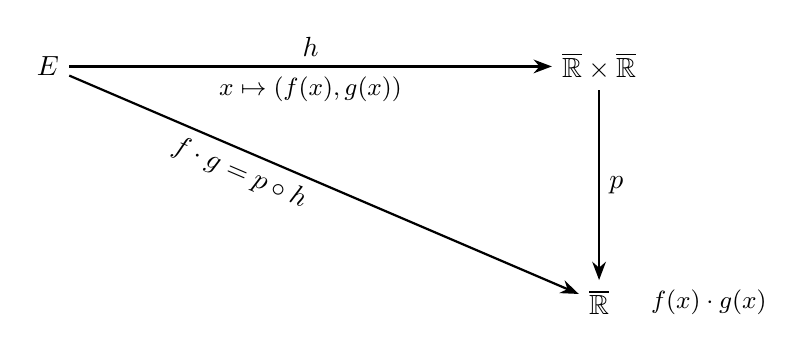
\begin{tikzpicture}[>=Stealth,thick,node distance=5cm]
  \node (E)  at (0,3) {$E$};
  \node (RR) at (7,3) {$\Rb\times\Rb$};
  \node (R)  at (7,0) {$\Rb$};
  \draw[->] (E) -- node[above]{$h$} node[below]{\small$x\mapsto(f(x),g(x))$} (RR);
  \draw[->] (RR) -- node[right]{$p$} (R);
  \draw[->] (E) -- node[below left,sloped]{$f\cdot g=p\circ h$} (R);
  \node[right=2pt of R,xshift=0.2cm,font=\small] {$f(x)\cdot g(x)$};
\end{tikzpicture}
\end{center}

Soit $x\in E$. Alors
\[
  (p\circ h)(x)=p\bigl(h(x)\bigr)=p\bigl(f(x),g(x)\bigr)=f(x)\cdot g(x)=(f\cdot g)(x).
\]
Dans le cas de $\R\times\R$, comme les pavés $[a,b]\times[c,d]$ engendrent $\B_{\R\times\R}$,
il suffit de montrer que
\[
  h^{-1}\bigl([a,b]\times[c,d]\bigr)\in\A .
\]
Or :
\begin{align*}
  h^{-1}\bigl([a,b]\times[c,d]\bigr)
    &=\bigl\{x\in E : h(x)\in[a,b]\times[c,d]\bigr\}\\
    &=\bigl\{x\in E : f(x)\in[a,b]\ \text{et}\ g(x)\in[c,d]\bigr\}\\
    &=f^{-1}\bigl([a,b]\bigr)\cap g^{-1}\bigl([c,d]\bigr)\in\A
\end{align*}
car $f$ et $g$ sont mesurables et $\A$ est une tribu.

%---------------------------------------------------------------------
\begin{enonce}{Théorème}{24}
Soit $(E,\A)$ un espace mesurable. Soit $f,g:E\to\Rb$ mesurables, alors
$f+g$, $f\cdot g$, $\alpha f\ (\alpha\in\R)$, $\sup(f,g)$, $\inf(f,g)$, $f^{+}$ et $f^{-}$ sont mesurables.
\end{enonce}

\begin{preuve}\end{preuve}

\textbf{1- Pour $f\cdot g : E\to\Rb$.} $f\cdot g$ est la composée de deux fonctions suivantes :
\[
  h:E\to\Rb\times\Rb,\ \ x\mapsto h(x)=\bigl(f(x),g(x)\bigr)
  \qquad\text{et}\qquad
  p:\Rb\times\Rb\to\Rb,\ \ (u,v)\mapsto u\cdot v .
\]
$h$ et $p$ étant mesurables, alors $f\cdot g=p\circ h$ est mesurable.

\textbf{2- Pour $f+g$ :} utiliser l'application de $E\to\Rb\times\Rb\setminus\{(-\infty,+\infty),(+\infty,-\infty)\}$.

\begin{note}
La preuve est seulement esquissée dans le manuscrit : on compose $h$ avec l'addition $(u,v)\mapsto u+v$,
mesurable sur $\Rb\times\Rb$ privé des deux couples ci-dessus.
\end{note}

\textbf{3- Pour $\sup(f,g)$.} $\sup(f,g)$ est la composée de :
\[
  h:E\to\Rb\times\Rb,\ \ x\mapsto h(x)=\bigl(f(x),g(x)\bigr)
  \qquad\text{et}\qquad
  S:\Rb\times\Rb\to\Rb,\ \ (u,v)\mapsto\sup(u,v).
\]
Donc $\sup(f,g)=S\circ h$. $h$ étant mesurable, il reste à montrer que
$S:(\Rb\times\Rb,\B_{\Rb\times\Rb})\to(\Rb,\B_{\Rb})$ est mesurable.

Or la famille des $\bigl([-\infty,a],\ a\in\R\bigr)$ engendre $\B_{\Rb}$, il suffit donc de montrer que
les $S^{-1}([-\infty,a])$ sont des mesurables (appartiennent à $\B_{\Rb\times\Rb}$). Or :
\[
  S^{-1}\bigl([-\infty,a]\bigr)=\bigl\{(x,y)\in\Rb\times\Rb : S(x,y)\in[-\infty,a]\bigr\}
  =[-\infty,a]\times[-\infty,a]\in\B_{\Rb\times\Rb}.
\]
Ainsi, $\sup(f,g)$ est mesurable.

\textbf{4- Pour $f^{+}$.} On a $f^{+}=\sup(f,0)$. Comme $f$ est mesurable et $0$ est mesurable,
alors $f^{+}$ est mesurable.

\begin{note}
Les cas $\inf(f,g)$, $\alpha f$ et $f^{-}$ ne sont pas détaillés dans le manuscrit.
Ils se traitent de même : $\inf(f,g)=-\sup(-f,-g)$ et $f^{-}=\sup(-f,0)$.
\end{note}

%---------------------------------------------------------------------
\begin{enonce}{Théorème}{25}
Soit $(f_n)$ une suite de fonctions numériques mesurables à valeurs dans $\Rb$, alors :
\begin{enumerate}[label=\textbf{\arabic*-},leftmargin=1.2cm]
  \item Les fonctions $\sup f_n$, $\inf f_n$, $\limsup f_n$ et $\liminf f_n$ sont mesurables.
  \item Si la suite $f_n$ converge simplement vers $f$, alors $f$ est mesurable.
\end{enumerate}
\end{enonce}

\begin{preuve}\end{preuve}

\textbf{1-} On a $\displaystyle\limsup f_n=\inf_{n\in\N}\Bigl(\sup_{p\ge n}f_p\Bigr)$.
On montre que $\limsup f_n$ est mesurable lorsqu'on a au préalable montré que
$\sup f_n$ et $\inf f_n$ sont mesurables.

Posons $g=\sup f_n : (E,\A)\to(\Rb,\B_{\Rb})$ avec $f_n$ mesurable.
Comme les $[-\infty,a]$ engendrent $\B_{\Rb}$, il suffit de montrer que
\[
  \forall a\in\R,\quad g^{-1}\bigl([-\infty,a]\bigr)\in\A .
\]
Soit $a\in\R$, alors :
\[
  g^{-1}\bigl([-\infty,a]\bigr)=\bigl\{x\in E : g(x)\in[-\infty,a]\bigr\}
  =\bigl\{x\in E : \sup_n f_n(x)\le a\bigr\}
  =\bigcap_{n\in\N} f_n^{-1}\bigl([-\infty,a]\bigr)\in\A
\]
car $f_n$ est mesurable et $\A$ est une tribu.

\begin{enonce}{Remarque}{26}
Ceci marche pour le $\sup$ ou le $\inf$ d'une famille dénombrable.
\end{enonce}

\begin{note}
Le manuscrit s'arrête ici : les preuves pour $\inf f_n$, $\limsup f_n$, $\liminf f_n$
et le point 2 du Théorème 25 ne sont pas écrites.
\end{note}

%=====================================================================
\section*{2-4) Fonctions étagées mesurables}

\begin{enonce}{Définition}{27}
\begin{enumerate}[label=\textbf{\arabic*-},leftmargin=1.2cm]
  \item Une application $f:E\to F$ est dite \emph{étagée} si elle prend un nombre fini de valeurs
        $(y_1,y_2,\dots,y_n)$ de $F$. Donc si $f(E)=\{y_1,y_2,\dots,y_n\}$.
  \item Si $\A$ est une famille de parties de $E$ ($\A\subset\Pp(E)$), $f:E\to F$ est dite
        \emph{étagée sur $\A$} si elle est étagée et si pour toute valeur $y_i\in F$ prise par $f$,
        $f^{-1}(\{y_i\})\in\A$.
\end{enumerate}
\end{enonce}

\begin{enonce}{Proposition}{28}
Pour qu'une application étagée $f:(E,\A)\to(\R,\B_{\R})$ soit mesurable,
il faut et il suffit qu'elle soit étagée sur $\A$.
\end{enonce}

\begin{preuve}\end{preuve}

($\Rightarrow$) \textit{Hypothèse :} $f$ est étagée et mesurable. Montrons que $f$ est étagée sur $\A$.
Soit $y_i\in\R$, alors $\{y_i\}$ est un borélien ; $f$ étant mesurable, alors $f^{-1}(\{y_i\})\in\A$.
D'où $f$ est étagée sur $\A$.

($\Leftarrow$) \textit{Hypothèse :} $f^{-1}(\{y_i\})\in\A$ pour $i=1,2,\dots,n$.
Montrons que $f$ est mesurable. Soit $A\in\B_{\R}$, a-t-on $f^{-1}(A)\in\A$ ? On a :
\[
  f^{-1}(A)=\bigcup_{y_i\in A} f^{-1}\bigl(\{y_i\}\bigr)\in\A
\]
car réunion finie d'éléments de $\A$, où $A=\bigcup_{y_i\in A}\{y_i\}$.

\begin{note}
Plus précisément, la réunion porte sur les $y_i\in A\cap f(E)$ : $f^{-1}(A)=f^{-1}(A\cap f(E))$.
Le symbole $A$ désigne ici un borélien et ailleurs la tribu $\A$ (notations proches dans le manuscrit).
\end{note}

%---------------------------------------------------------------------
\begin{enonce}{Proposition}{29}
L'ensemble des fonctions étagées sur la $\sigma$-algèbre $\A$ et à valeurs dans $\R$
est un espace vectoriel $\Ee(\A,\R)$.
\end{enonce}

\begin{preuve}\end{preuve}

Soit $f(E)=\{y_1,y_2,\dots,y_n\}$ et $g(E)=\{z_1,z_2,\dots,z_p\}$.
Alors $f+g$ prend des valeurs dans l'ensemble fini $\{y_i+z_j\}_{\,i=1,\dots,n;\ j=1,\dots,p}$.

Soit $x$ une valeur prise par $f+g$ ; on veut montrer que $(f+g)^{-1}(x)\in\A$.
Il y a un nombre fini de couples $(i,j)$ tels que $y_i+z_j=x$, et
$f^{-1}(\{y_i\})\cap g^{-1}(\{z_j\})\in\A$ car $f$ et $g$ sont étagées sur $\A$ et $\A$ est une tribu.
Ainsi :
\[
  \bigcup_{(i,j)\in I}\Bigl(f^{-1}(\{y_i\})\cap g^{-1}(\{z_j\})\Bigr)\in\A,
  \qquad\text{où } I=\bigl\{(i,j) : y_i+z_j=x\bigr\}.
\]
D'où $(f+g)^{-1}(x)\in\A$.

\begin{note}
Seule la stabilité par addition est écrite dans le manuscrit ;
la stabilité par multiplication par un scalaire ($\lambda f$) se traite de la même façon.
\end{note}

%---------------------------------------------------------------------
\begin{enonce}{Théorème}{30}
Soit $(E,\A)$ un espace mesurable. Toute fonction mesurable positive (à valeurs dans $\overline{\R_+}$)
est limite d'une suite croissante de fonctions étagées positives sur $\A$.
\end{enonce}

\begin{preuve}\end{preuve}

Soit $f:E\to\overline{\R_+}$ mesurable. Construisons une suite $(f_n)$ croissante de fonctions étagées
et positives qui tend vers $f$.

\begin{center}
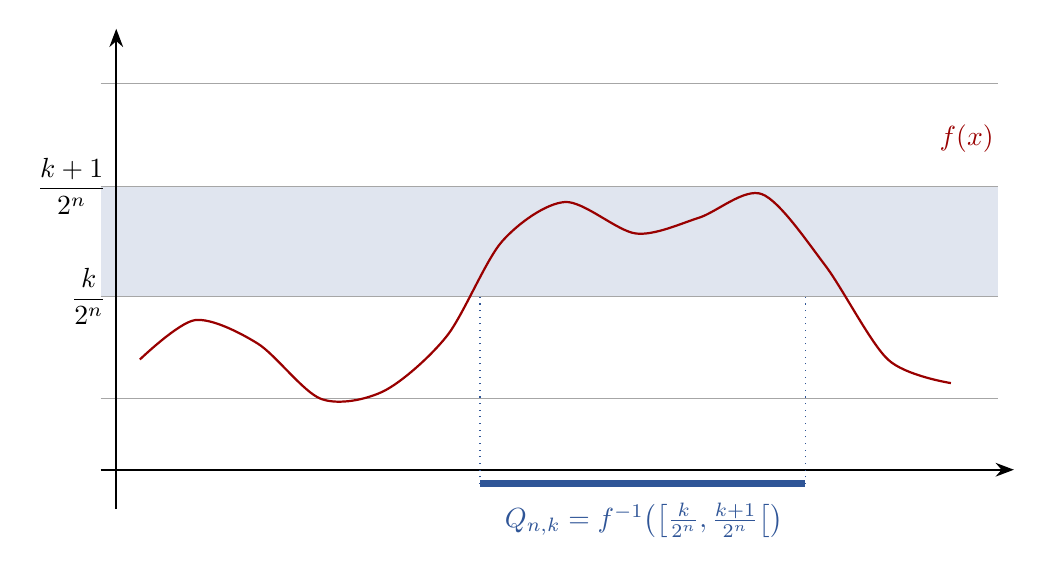
\begin{tikzpicture}[scale=1,>=Stealth]
  % bande [k/2^n,(k+1)/2^n[
  \fill[bleuclair!15] (-0.2,2.2) rectangle (11.2,3.6);
  \foreach \y in {0.9,2.2,3.6,4.9}{\draw[gray!70,thin] (-0.2,\y) -- (11.2,\y);}
  % axes
  \draw[->,thick] (-0.2,0) -- (11.4,0);
  \draw[->,thick] (0,-0.5) -- (0,5.6);
  % graphe de f
  \draw[thick,red!60!black,smooth] plot coordinates
    {(0.3,1.4)(1.0,1.9)(1.8,1.6)(2.6,0.9)(3.4,1.0)(4.2,1.7)(4.9,2.9)(5.7,3.4)(6.6,3.0)(7.4,3.2)(8.2,3.5)(9.0,2.6)(9.8,1.4)(10.6,1.1)};
  % étiquettes
  \node[left] at (0,2.2) {$\dfrac{k}{2^n}$};
  \node[left] at (0,3.6) {$\dfrac{k+1}{2^n}$};
  \node[red!60!black] at (10.8,4.2) {$f(x)$};
  % Q_{n,k}
  \draw[bleuclair,line width=2.5pt] (4.62,-0.18) -- (8.75,-0.18);
  \draw[bleuclair,dotted] (4.62,-0.18) -- (4.62,2.2);
  \draw[bleuclair,dotted] (8.75,-0.18) -- (8.75,2.2);
  \node[bleuclair,below] at (6.7,-0.3) {$Q_{n,k}=f^{-1}\!\left(\left[\frac{k}{2^n},\frac{k+1}{2^n}\right[\right)$};
\end{tikzpicture}
\end{center}

On construit $(f_n)$ de la manière suivante.
\begin{itemize}[leftmargin=1.2cm]
  \item Dans $R_n=f^{-1}\bigl([n,+\infty]\bigr)$, on pose : $f_n(x)=n$.
  \item Dans chaque $Q_{n,k}=f^{-1}\Bigl(\Bigl[\dfrac{k}{2^n},\dfrac{k+1}{2^n}\Bigr[\Bigr)$, on pose :
        $f_n(x)=\dfrac{k}{2^n}$ \quad (lorsque $\dfrac{k}{2^n}\le f(x)<\dfrac{k+1}{2^n}$).
\end{itemize}
Alors $0\le k\le n\times 2^n$.

\begin{note}
Le manuscrit écrit « $f_n(x)=n$ ($x\ge n$) » et « $\frac{k}{2^n}\le x<\frac{k+1}{2^n}$ » :
c'est en réalité $f(x)$ qui intervient (et non $x$). De plus, avec ces intervalles semi-ouverts,
on a $0\le k\le n\,2^n-1$.
\end{note}

\textbf{1-} Les premiers points sont étagés sur $\A$ car $Q_{n,k}$ et $R_n\in\A$.

\textbf{2-} Montrons que la suite $(f_n)$ est croissante. Il suffit de montrer que dans chaque domaine
$Q_{n,k}$, $R_n$ on a : $f_n(x)\le f_{n+1}(x)$.

On a :
\[
  \Bigl[\frac{k}{2^n},\frac{k+1}{2^n}\Bigr[
  =\Bigl[\frac{2k}{2^{n+1}},\frac{2k+1}{2^{n+1}}\Bigr[\ \cup\ \Bigl[\frac{2k+1}{2^{n+1}},\frac{2k+2}{2^{n+1}}\Bigr[
\]
Donc $Q_{n,k}=Q_{n+1,2k}\cup Q_{n+1,2k+1}$.

Si $x\in R_n$ : $[n,+\infty]=[n,n+1[\ \cup\ [n+1,+\infty]$, soit
\[
  [n,+\infty]=\Biggl(\bigcup_{n\times 2^{n+1}\,\le\,k\,\le\,(n+1)2^{n+1}}
  \Bigl[\frac{k}{2^{n+1}},\frac{k+1}{2^{n+1}}\Bigr[\Biggr)\ \cup\ [n+1,+\infty].
\]
Ainsi :
\[
  R_n=\Biggl(\bigcup_{n\times 2^{n+1}\,\le\,k\,\le\,(n+1)2^{n+1}} Q_{n+1,k}\Biggr)\cup R_{n+1},
\]
où, selon le cas :
\begin{itemize}[leftmargin=1.2cm]
  \item $f_{n+1}(x)=\dfrac{k}{2^{n+1}}\ \ge\ n=f_n(x)$ ;
  \item ou bien $f_{n+1}(x)=n+1>n=f_n(x)$.
\end{itemize}
Donc $f_n$ est croissante.

\begin{note}
Dans la réunion, $k$ doit aller de $n\,2^{n+1}$ à $(n+1)\,2^{n+1}-1$ pour que les $Q_{n+1,k}$
soient bien contenus dans $R_n$.
\end{note}

\textbf{3-} Montrons que $f_n\to f$ simplement.

\emph{1\textsuperscript{er} cas :} si $f(x)\neq+\infty$, alors $\exists\, n_0\in\N$ tel que $n_0>f(x)$.
Pour $n\ge n_0$, $x\in Q_{n,k}$ tel que
\[
  \frac{k}{2^n}\le f(x)<\frac{k+1}{2^n}\qquad\text{et}\qquad f_n(x)=\frac{k}{2^n},
\]
ainsi $f(x)-f_n(x)<\dfrac{1}{2^n}\xrightarrow[n\to+\infty]{}0$.

\emph{2\textsuperscript{e} cas :} si $f(x)=+\infty$, alors $\forall n$, $x\in R_n$, donc
$f_n(x)=n\xrightarrow[n\to+\infty]{}+\infty=f(x)$.

Ainsi, $f_n(x)\to f(x)$.

%---------------------------------------------------------------------
\begin{enonce}{Corollaire}{31}
Soit $(E,\A)$ un espace mesurable. Toute fonction numérique mesurable est limite simple
d'une suite de fonctions étagées sur $\A$ à valeurs dans $\R$.
\end{enonce}

\begin{preuve}\end{preuve}

On écrit $f=f^{+}-f^{-}$, et $f^{+}$ et $f^{-}$ sont des fonctions mesurables positives.
On peut leur appliquer le théorème précédent.

Donc il existe une suite croissante $(g_n)$ de fonctions étagées positives sur $\A$ telle que
$g_n\to f^{+}$. De même, il existe une suite croissante $(h_n)$ de fonctions étagées positives
sur $\A$ telle que $h_n\to f^{-}$.

$g_n-h_n$ est étagée sur $\A$ et à valeurs dans $\R$, et
\[
  g_n-h_n\longrightarrow f^{+}-f^{-}=f .
\]

\begin{note}
« Étagée sur $\A$ » résulte de la Proposition 29 (espace vectoriel).
\end{note}

\end{document}
